\documentclass{article}

\usepackage{amsmath, graphicx}

\graphicspath{ {./images/} }

\title{Ch. 27 HW \#2 Solutions}
\author{Principles of Macroeconomics}
\date{today}

\begin{document}

\maketitle

\section*{Questions for Review}

\begin{enumerate}

\setcounter{enumi}{4}

\item A decrease in the tax on interest earnings will make saving more lucrative. That will incentivize households to save more, so private saving increases. Importantly, we have to assume that the increase in private saving is larger than the decrease in public saving due to the decrease in tax revenue.

In the market for loanable funds, an increase in saving shifts supply right, drives the interest rate down, and increases the quantity of investment in the economy.

	\begin{center}
	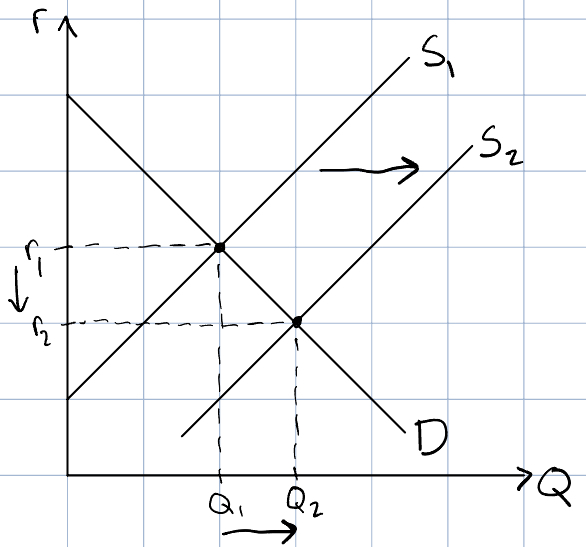
\includegraphics[width = 0.5\textwidth]{qfr5}
	\end{center}
	
\item A government budget deficit occurs when the government spends more than it collects in tax revenue. It decreases public saving which shifts the supply of loanable funds to the left. That in turn increases the interest rate and decreases the quantity of investment in the economy.

	\begin{center}
	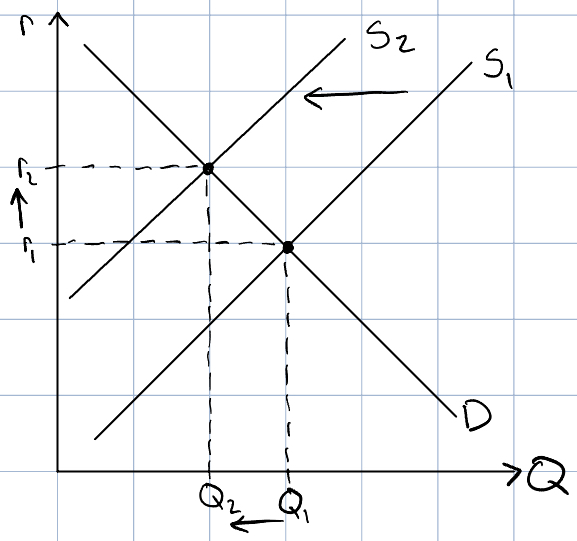
\includegraphics[width = 0.5\textwidth]{qfr6}
	\end{center}
Lower investment leads to slower growth in the capital stock. Lower growth in the capital stock leads to slower economic growth.

\end{enumerate}



\section*{Problems and Applications}

\begin{enumerate}

\setcounter{enumi}{4}

\item \begin{gather*}
	S_{Priv} = Y - T - C = 10,000 - 1,500 - 6,000 = 2,500 \\
	S_{Pub} = T - G = 1,500 - 1,700 = -200 \\
	S_{Nat} = S_{Priv} + S_{Pub} = 2,500 - 200 = 2,300 \\
	I = S_{Nat} = 2,300
	\end{gather*}
	\begin{align*}
	I &= 3,300 - 100r \\
	2,300 &= 3,300 - 100r \\
	100r &= 1,000 \\
	r &= 10\%
	\end{align*}
	
\item

	\begin{enumerate}
	
	\item Higher interest rates make it more expensive for Intel to borrow money for the factory. That makes them less likely to build the factory. 
	
	\item It would. Higher interest rates make it more lucrative for Intel to save its money rather than spend it. That makes them more likely to save and less likely to build the factory.
	
	\end{enumerate}
	
\item

	\begin{enumerate}
	
	\item Harry: \$1,000(1.05) = \$1,050 \\
		Ron: \$1,000(1.08) = \$1,080 \\
		Hermione \$1,000(1.20) = \$1,200
		
	\item If the rate of return on their investment is greater than $r$, then they would borrow because they would make more money on the investment than they would spend on interest. If the rate of return on their investment is lower than $r$, then they would lend because they would make more money from interest than they would on the investment.
	
	\item At 7\%, Ron and Hermione would both want to borrow, so the quantity of loanable funds demanded would be \[ \$1,000 + \$1,000 = \$2,000. \] Harry would want to save, so the quantity of loanable funds supplied would be \$1,000. \\
	At 10\%, Hermione would want to borrow, so the quantity of loanable funds demanded would be \$1,000. Harry and Ron would both want to save, so the quantity of loanable funds supplied would be \[\$1,000 + \$1,000 = \$2,000. \]
	
	\item At an interest rate of 8\%, the market for loanable funds would be at equilibrium. Harry would want to lend \$1,000, and Hermione would want to borrow \$1,000. Ron would be indifferent between borrowing and lending, so he would likely do neither and just invest his own money. 
	
	\item Harry: \$1,000(1.08) = \$1,080 \\
		Ron: \$1,000(1.08) = \$1,080 \\
		Hermione: \$2,000(1.20) - \$1,000(1.08) = \$2,400 - \$1,080 = \$1,320
		
		Harry and Hermione both benefit from loanable funds market because they make more money than they would without it. Ron is just as well off as he would be  without it, so no one's worse off.
	
	\end{enumerate}

\end{enumerate}

\end{document}